\documentclass{article}
\usepackage{amsmath}
\usepackage{amssymb}
\usepackage{graphicx}
\usepackage{hyperref}
\usepackage[version=4]{mhchem}

\title{Example 18}
\date{}

\begin{document}
\maketitle

In \(A B C, E\) is a point on \(A B\) and \(F\) is a point on \(A C\) such that \(\angle F B C\) \(=\angle E C B=\frac{1}{2} \angle A\). Prove: \(B E=C F\).

Proof:
Draw \(B G \perp C E\) to meet \(C E\) at \(G\).\\
\centering
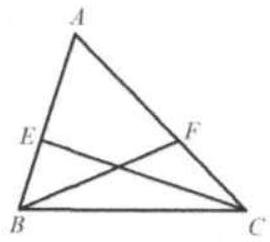
\includegraphics[width=\textwidth]{images/085(2).jpg}

Draw \(C H \perp B F\) to meet the extension of \(B F\) at \(H\).\\
\(\triangle B G C \cong \triangle C H B\left(B C=B C, \angle B G C=\angle C H B=90^{\circ}, \angle H B C=\angle G C B\right)\), then \(B G\) \(=\mathrm{CH}\).\\
\centering
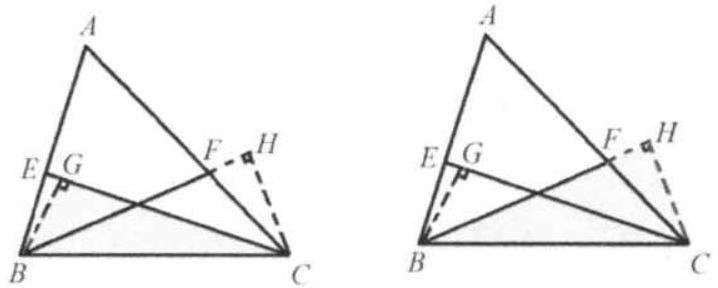
\includegraphics[width=\textwidth]{images/085(1).jpg}\\
\(\angle B E G=\angle A+\angle A C E=\angle F B C+\angle A C E+\angle E C B\)\\
\(\angle C F H=\angle A F B=\angle F B C+\angle A C E+\angle E C B\)

Thus \(\angle B E G=\angle C F H\).\\
So we get \(\triangle B E G \cong \triangle C F H\left(\angle B E G=\angle C F H, \angle B G E=\angle C H F=90^{\circ}, B G=C H\right)\), and \(B E=C F\).\\
\centering
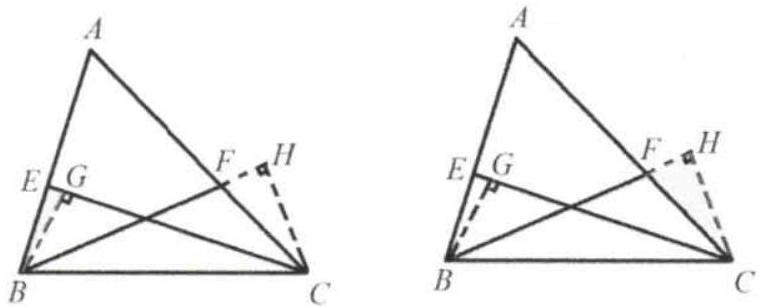
\includegraphics[width=\textwidth]{images/085.jpg}



\end{document}
